\documentclass[hyperref={pdfpagelabels=false}]{beamer}

\usepackage{listings}
\usetheme{default}
\setbeamercovered{transparent}
\setbeamertemplate{footline}[page number]
\setbeamertemplate{navigation symbols}{} %remove navigation symbols

\newcommand{\codestyle}{\small\sffamily}

% "define" Scala
\lstdefinelanguage{scala}{
  alsoletter={@,=,>},
  morekeywords={abstract, case, catch, class, def, do, else, extends, false, final, finally, for, if, implicit, import, match, new, null, object, 
override, package, private, protected, requires, return, sealed, super, this, throw, trait, try, true, type, val, var, while, with, yield, domain, 
postcondition, precondition,invariant, constraint, assert, forAll, in, _, return, @generator, ensure, require, holds, ensuring,=>},
  sensitive=true,
  morecomment=[l]{//},
  morecomment=[s]{/*}{*/},
  morestring=[b]"
}
\lstset{
%  frame=tb,
  language=scala,
%  aboveskip=3mm,
%  belowskip=3mm,
%  lineskip=-0.1em,
  showstringspaces=false,
  columns=fullflexible,
  mathescape=true,
  numbers=none,
  numberstyle=\tiny,
  basicstyle=\codestyle
} 

\begin{document}
\title{Toward Interprocedural Pointer and Effect Analysis for Scala}
\author{Etienne Kneuss}
\date{\today}

\institute[EPFL]{
Laboratory for Automated Reasoning and Analysis \\
School of Computer and Communication Sciences\\
EPFL
}

\begin{frame}
    \titlepage
\end{frame}

\section*{Outline}
\begin{frame}
    \frametitle{Outline}
    \tableofcontents
\end{frame}

\section{Introduction}
%\begin{frame}
%    \frametitle{Scala}
%    \begin{itemize}
%        \item Growing language
%        \item Lorem ipsum
%        \item Lorem ipsum
%    \end{itemize}
%\end{frame}

\begin{frame}[label=overview]
%    \frametitle{INSANE}
    \begin{figure}[t]
        
\includegraphics[width=60mm]{../../logo.png}\\
        Interprocedural Static Analysis Engine for Scala
    \end{figure}

    \begin{itemize}
        \item Precise pointer and effect analysis
            \begin{itemize}
                \item Whole-Program but compositional
                \item Based on abstract interpretation
                \item Interprocedural
            \end{itemize}
        \item Working Implementation
            \begin{itemize}
                \item Provided as a compiler plug-in
                \item Accepts any Scala code
                \item Requires no annotations
            \end{itemize}
    \end{itemize}
\end{frame}

\begin{frame}
\frametitle{Definitions}
    \textbf{Pointer Analysis}\\
    \emph{Static analysis technique that builds information on the
relations between pointers and allocated objects.}

    \vspace{30pt}

    \textbf{Effect Analysis}\\
    \emph{Static analysis technique that summarizes the side effects
of procedures in a certain domain.}
\end{frame}

\begin{frame}
    \frametitle{Analysis Phases}
    The analysis currently consists of three main phases:
    \begin{enumerate}
        \item Type/Class Analysis \& Call Graph Generation
        \item Effect Graphs Generation
        \item Purity Analysis
\end{enumerate}

\end{frame}

\begin{frame}[fragile]
\frametitle{Type/Class Analysis}

    Type/Class Analysis aims at establishing the types of runtime values. In
    the presence of dynamic dispatch, this information is used to compute a
    precise call-graph.

    \begin{columns}
      \begin{column}{0.5\textwidth}
\begin{lstlisting}
object Test {
    def run1(obj: A) {
        obj.f()
    }
    def run2() {
        val obj = new A
        obj.f()
    }
}
\end{lstlisting}
      \end{column}
      \begin{column}{0.5\textwidth}
\begin{lstlisting}
class A {
    def f() { ... }
}
class B extends A {
    def f() { ... }
}
\end{lstlisting}
      \end{column}
    \end{columns}


\end{frame}

\begin{frame}[fragile]
    \frametitle{Type/Class Analysis}
    \begin{itemize}
        \item Analysis is flow sensitive, based on abstract interpretation
        \item Abstract values are of the form:
$$ \langle T_{sub}, T_{exact} \rangle $$
where $T_{sub}$ and $T_{exact}$ are two sets of types
    \end{itemize}

\begin{figure}
    \begin{tabular}{ l | l }
        Expression $ex$       & Abstract Value $\alpha(ex)$\\
        \hline
        \verb/new A/          & $\langle \emptyset, \{ A \} \rangle$ \\
        \verb/null/           & $\langle \emptyset, \emptyset \rangle$ \\
        \verb/obj.f/            & $\langle\{type(\verb/obj.f/)\}, \{type(\verb/obj.f/)\} \rangle$ \\
        \verb/rec.meth(..)/   & $\langle\{type(\verb/rec.meth/)\}, \{type(\verb/rec.meth/)\} \rangle$ \\
    \end{tabular}
\end{figure}
\end{frame}

\section{Analysis}
\begin{frame}
\end{frame}

\begin{frame}[fragile]
    \frametitle{Purity Analysis}
    \begin{itemize}
        \item Checks for observable purity
            \begin{itemize}
                \item Look for inside edges (writes) reachable from nodes
accessible from \emph{outside} (PNodes, OBNodes, ...)
            \end{itemize}
        \item If not pure, computes \emph{modifies clauses}
    \end{itemize}

    \begin{columns}
      \begin{column}{0.5\textwidth}
\begin{lstlisting}
class Counter {
  var v = 0
}

class Test1 {
  def fun() {
    val localC = new Counter
    localC.v = 42
  }
}
\end{lstlisting}
      \end{column}
      \begin{column}{0.5\textwidth}
\begin{lstlisting}
class Test2 {
  val c = new Counter
  def fun() {
    c.v = 42
  }
}
\end{lstlisting}
      \end{column}
    \end{columns}
\end{frame}

\begin{frame}[fragile]
    \frametitle{Purity Analysis}
    \begin{columns}
      \begin{column}{0.4\textwidth}
\begin{lstlisting}
class Test1 {
  def fun() {
    val localC = new Counter
    localC.v = 42
  }
}
\end{lstlisting}
        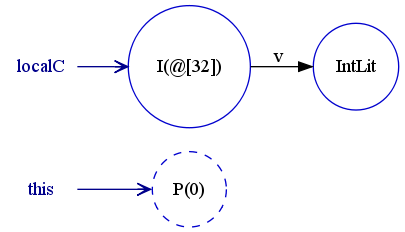
\includegraphics[width=40mm]{images/purity_fun1_pt.png}
%        \vspace{10pt}
%        \lstinline{Test1.fun: @Pure}
      \end{column}
      \begin{column}{0.6\textwidth}
\begin{lstlisting}
class Test2 {
  val c = new Counter
  def fun() {
    c.v = 42
  }
}
\end{lstlisting}
        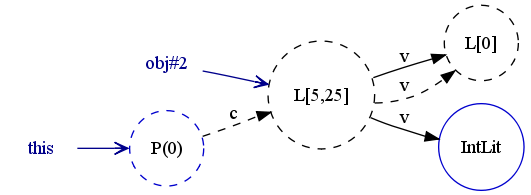
\includegraphics[width=50mm]{images/purity_fun2_pt.png}

%        \vspace{10pt}
%        \lstinline{Test2.fun: @Modifies(this.c.v)}
      \end{column}
    \end{columns}
\end{frame}
\begin{frame}[fragile]
    \frametitle{Purity Analysis}
    \begin{columns}
      \begin{column}{0.4\textwidth}
\begin{lstlisting}
class Test1 {
  def fun() {
    val localC = new Counter
    localC.v = 42
  }
}
\end{lstlisting}
        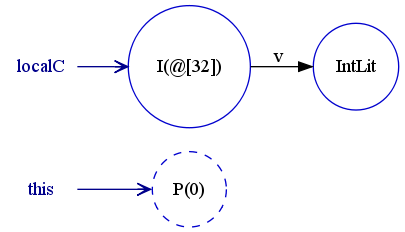
\includegraphics[width=40mm]{images/purity_fun1_pt.png}
        \vspace{10pt}
        \lstinline{Test1.fun: @Pure}
      \end{column}
      \begin{column}{0.6\textwidth}
\begin{lstlisting}
class Test2 {
  val c = new Counter
  def fun() {
    c.v = 42
  }
}
\end{lstlisting}
        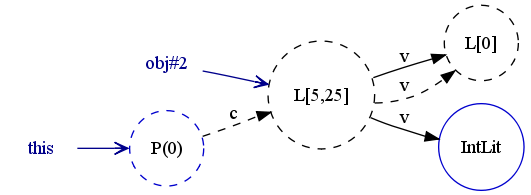
\includegraphics[width=50mm]{images/purity_fun2_pt.png}

        \vspace{10pt}
        \lstinline{Test2.fun: @Modifies(this.c.v)}
      \end{column}
    \end{columns}
\end{frame}

\section{Implementation}
\begin{frame}
\end{frame}

\section{Limitations and Future Work}
\begin{frame}
\end{frame}

\section{Related Work}
\begin{frame}
\end{frame}

\section{Conclusion}
\againframe{overview}

\section*{Thanks}
\begin{frame}
    \begin{center}
        Thanks!
    \end{center}
\end{frame}
\appendix
\newcounter{finalframe}
\setcounter{finalframe}{\value{framenumber}}

\begin{frame}
\end{frame}

\begin{frame}
    Additional Material
\end{frame}
\setcounter{framenumber}{\value{finalframe}}
\end{document}
